\begin{flushright}
\begin{tabular}{l}
{\em Something unknown is doing we don't know what.}\\
\ \ \ \ -- Sir Arthur Eddington
\end{tabular}
\end{flushright}

\section{Introduction}
\label{sec:intro}   

Intelligence is a multifaceted and elusive concept that has long challenged psychologists, philosophers, and computer scientists.
An attempt to capture its essence was made in 1994 by a group of 52 psychologists who signed onto a broad definition published in an editorial about the science of intelligence~\cite{gottfredson1997mainstream}.
The consensus group defined intelligence as {\em a very general mental capability that, among other things, involves the ability to reason, plan, solve problems, think abstractly, comprehend complex ideas, learn quickly and learn from experience}.
This definition implies that intelligence is not limited to a specific domain or task, but rather encompasses a broad range of cognitive skills and abilities.
Building an artificial system that exhibits the kind of general intelligence captured by the 1994 consensus definition is a long-standing and ambitious goal of AI research.
In early writings, the founders of the modern discipline of artificial intelligence (AI) research called out sets of aspirational goals for understanding intelligence~\cite{mccarthy2006proposal}.
Over decades, AI researchers have pursued principles of intelligence, including generalizable mechanisms for reasoning (e.g.,~\cite{newellshawsimonGPS1959},~\cite{lindsay1993dendral}) and construction of knowledge bases containing large corpora of commonsense knowledge~\cite{lenat1995cyc}.
However, many of the more recent successes in AI research can be described as being narrowly focused on well-defined tasks and challenges, such as playing chess or Go, which were mastered by AI systems in 1996 and 2016, respectively. In the late-1990s and into the 2000s, there were increasing calls for developing more general AI systems (e.g.,~\cite{selman1996challenge}) and scholarship in the field has sought to identify principles that might underly more generally intelligent systems (e.g.,~\cite{legg2008machine, gershman2015computational}). The phrase, ``artificial general intelligence" (AGI), was popularized in the early-2000s (see~\cite{goertzel2014artificial}) to emphasize the aspiration of moving from the ``narrow AI", as demonstrated in the focused, real-world applications being developed, to broader notions of intelligence, harkening back to the long-term aspirations and dreams of earlier AI research.
We use AGI to refer to systems that demonstrate broad capabilities of intelligence as captured in the 1994 definition above, with the additional requirement, perhaps implicit in the work of the consensus group, that these capabilities are at or above human-level. We note however that there is no single definition of AGI that is broadly accepted, and we discuss other definitions in the conclusion section.
%from the literature in Section~\ref{sec:otherdefinitions}.
\newline 

The most remarkable breakthrough in AI research of the last few years has been the advancement of natural language processing achieved by large language models (LLMs). These neural network models are based on the Transformer architecture~\cite{Vas17} and trained on massive corpora of web-text data, using at its core a self-supervised objective of predicting the next word in a partial sentence.
In this paper, we report on evidence that a new LLM developed by OpenAI, which is an early and \textbf{non-multimodal} version of \DV\ \cite{gpt4}, exhibits many traits of intelligence, according to the 1994 definition. 
Despite being purely a language model, this early version of {\DV} demonstrates remarkable capabilities on a variety of domains and tasks, including abstraction, comprehension, vision, coding, mathematics, medicine, law, understanding of human motives and emotions, and more. 
%March 13th edits:
We interacted with \DV\ during its early development by OpenAI using purely natural language queries (prompts)\footnote{As \DV’s development continued after our experiments, one should expect different responses from the final version of \DV. In particular, all quantitative results should be viewed as estimates of the model’s potential, rather than definitive numbers. We repeat this caveat throughout the paper to clarify that the experience on the deployed model may differ. Moreover we emphasize that the version we tested was text-only for inputs, but for simplicity we refer to it as \DV\ too.}.
%We interact with {\DV} using natural language queries (prompts), and we observe its responses and behaviors. 
In Figure~\ref{fig:prelimexamples}, we display some preliminary examples of outputs from {\DV}, asking it to write a proof of infinitude of primes in the form of a poem, to draw a unicorn in TiKZ (a language for creating graphics in \LaTeX), to create a complex animation in Python, and to solve a high-school level mathematical problem. It easily succeeds at all these tasks, and produces outputs that are essentially indistinguishable from (or even better than) what humans could produce. We 
also compare \DV's performance to those of previous LLMs, most notably ChatGPT, which is a fine-tuned version of (an improved) GPT-3~\cite{gpt3}. In Figure~\ref{fig:prelimexamplesChatGPT}, we display the results of asking ChatGPT for both the infinitude of primes poem and the TikZ unicorn drawing. While the system performs non-trivially on both tasks, there is no comparison with the outputs from \DV. These preliminary observations will repeat themselves throughout the paper, on a great variety of tasks. The combination of the generality of \DV's capabilities, with numerous abilities spanning a broad swath of domains, and its performance on a wide spectrum of tasks at or beyond human-level, makes us comfortable %with calling {\DV} an {\em AGI system}
with saying that {\DV} is a significant step towards AGI.
%\footnote{
%Importantly, we stop short of referring to {\DV} as \textbf{AGI} due to the many limitations which we shall discuss extensively, including the lack of true real-time learning.}.
\newline

\begin{figure}
\begin{AIbox}{\DV}
\parbox[t]{0.55\linewidth}{
{\small {\bf Prompt:} Can you write a proof that there are infinitely many primes, with every line that rhymes?}\\

{\small\bf \DV:} \scriptsize \begin{alltt}
Yes, I think I can,

Though it might take a clever plan. 

I'll start by noting Euclid's proof, 

Which shows that primes aren't just aloof. 

Assume we have a finite list, 

Of primes, and that none have been missed. 

Multiply them all together, 

And add one, just to be clever. 

The result will be a number, 

That has no prime factors, oh wonder! 

But every number has a prime, 

That divides it, it's just a matter of time. 

So we've found a contradiction, 

And our finite list needs eviction. 

There must be infinitely many primes, 

And that's the end of my rhyming lines.s
\end{alltt}}
\hspace{0.2in}
\parbox[t]{0.4\linewidth}{\small {\bf Prompt:} Draw a unicorn in TiKZ.\\\ \\

{\bf \DV:}
{\scriptsize [Produces \LaTeX\ compiling to following picture.]} \\
%\vspace{1in}

\drawunicorn{1.2}
}
\tcbline
{\small \bf Prompt:} {\scriptsize Can you generate a pyplot for the following data: $x = [1, 3, 5, 6, 8], y1 = [2, 3, 5, 18, 1], y2 = [3, 5, 6, 8, 1], y3 = [5, 1, 2, 3, 4], y4 = [9, 7, 2, 3,  1].$ I want $y1, y2$ to be in the same plot, but $y3$ is in another plot next to that plot, $y4$ is in below. I want the legend of $y1$ to be "bob", $y2$ to be "alice", $y3$ to be "bilbo", $y4$ to be "allie".
I want the $x$-axis to be labeled with "time" and $y$ axis to be labeled with "money".
I want to add a 10 \%-40\% random error bar to each curve, through all times (including non-integers).
I want smoothed curves to show the plot, and smoothed error bar. Do not use linear interpolation, use smooth interpolation!
I want to also add some small zig-zag to the smoothed curve to make it look more real.
I want to put a baseline as the mean of each line.
I want to put a pie chart below indicating the fraction of the four people in each time step.
I also want an animation to show how the fractions are changing in the pie chart in **continuous time**. Interpolate the missing fractions!
I also want vertical line animation in other three plots to match the pie chart.
I want the fanciest plot. Please add as many fancy things as possible.

Here is a possible code to generate a pyplot for the following data, with some comments to explain the steps:} \\

{\small \bf \DV:} {\scriptsize [We give two snapshots from the animation resulting from the produced code]} \\

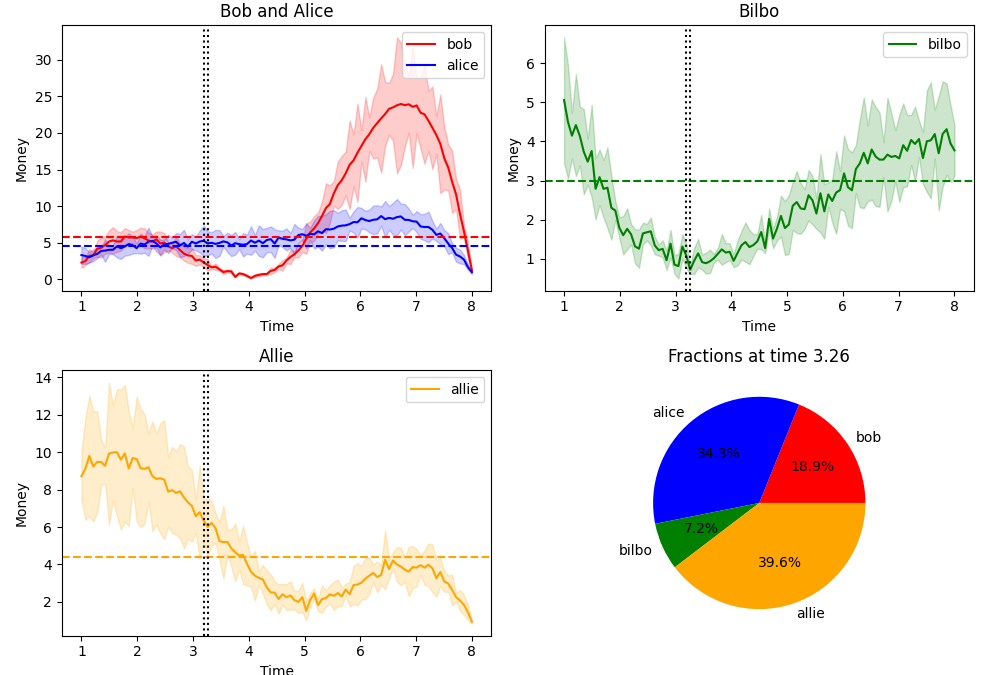
\includegraphics[width=0.49\textwidth]{figures/ff_1.png}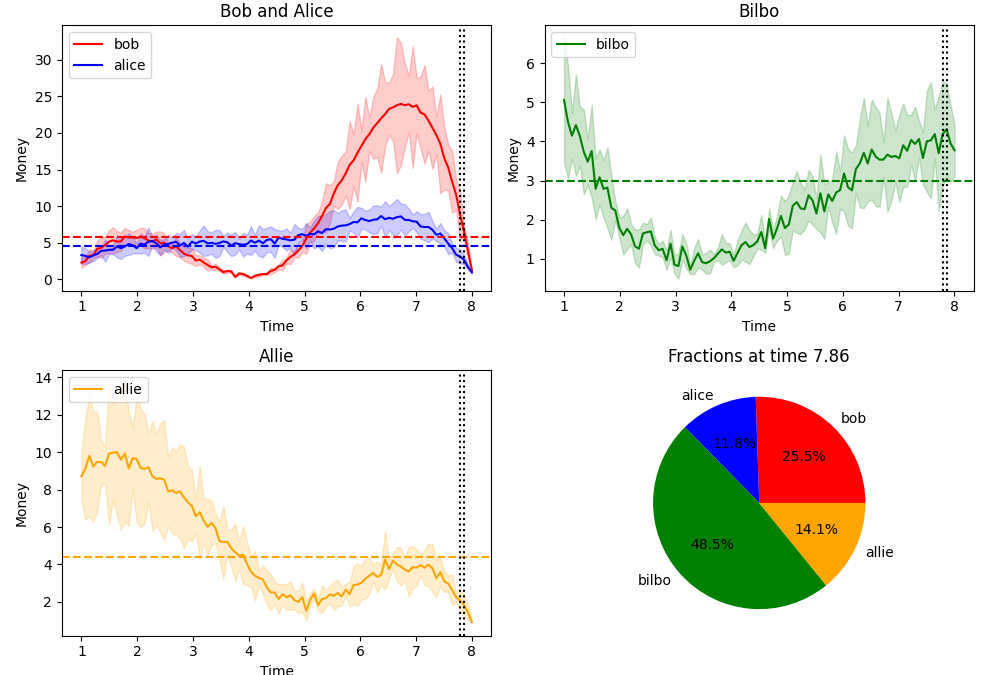
\includegraphics[width=0.49\textwidth]{figures/ff_2.png}

\tcbline
{\small \bf Prompt:} {\scriptsize Suppose $g(x) = f^{-1}(x), g(0) = 5, g(4) = 7, g(3) = 2, g(7) =  9, g(9) = 6$ what is $f(f(f(6)))$?} \\

{\small \bf \DV:} {\scriptsize There are different ways to approach this problem, but one possible method is to use the fact that $g(x) = f^{-1}(x)$ implies that $f(g(x)) = x$ for any $x$ in the domain of $g$. That is, applying $f$ to both sides of the equation $g(x) = f^{-1}(x)$ gives $f(g(x)) = f(f^{-1}(x)) = x$. This means that we can undo the effect of $f$ by applying $g$, and vice versa. Using this idea, we can try to find $f(6)$ by looking for the value of $x$ such that $g(x) = 6$. From the given information, we see that $g(9) = 6$, so $f(6) = f(g(9)) = 9$. Similarly, we can find $f(9)$ by looking for the value of $x$ such that $g(x) = 9$. We see that $g(7) = 9$, so $f(9) = f(g(7)) = 7$. Finally, we can find $f(7)$ by looking for the value of $x$ such that $g(x) = 7$.  We see that $g(4) = 7$, so $f(7) = f(g(4)) = 4$. Therefore, $f(f(f(6))) = f(f(9)) = f(7) = 4$.}
\end{AIbox}
\caption{Preliminary examples of {\DV}'s capabilities in language, vision, coding, and mathematics.}
\label{fig:prelimexamples}
\end{figure}

\begin{figure}

\begin{AIbox}{ChatGPT}
\parbox[t]{0.6\linewidth}{
{\small {\bf Prompt:} Can you write a proof that there are infinitely many primes, with every line that rhymes?}\\

{\small\bf ChatGPT:} \scriptsize \begin{alltt}
Sure! Here is a proof that there are infinitely many primes, with each line of the proof rhyming:
\\

Consider the set of all primes.

Call this set P and let it start with just two, the first prime.

If we take all the primes in P and add one,

We get a new set of numbers that has never been done.
\\

This set, call it S, is composed of only composite numbers.

No primes will be found among them, that's for sure.

But we know that there must be at least one prime,

Since S is infinite, and that much is clear.
\\

If we take the smallest number in S that is not in P,

And call it p, we can add it to our set, don't you see?

But this process can be repeated indefinitely.

Thus, our set P must also be infinite, you'll agree.
\\

So there you have it, a proof that's quite solid.

There are infinitely many primes, that much we can see.

No need to be coy, no need to be contrite.

Infinity is a big number, just like P.
\end{alltt}}
\hspace{0.2in}
\parbox[t]{0.35\linewidth}{\small {\bf Prompt:} Draw a unicorn in TiKZ.\\

{\bf ChatGPT:} {\scriptsize [Produces \LaTeX\ compiling to following picture.]} \\

\vspace{0.3in}

\begin{tikzpicture}
\hspace{-0.5in}
\begin{scope}
    \clip(-2.5,-1) rectangle (3,2.5);
    % Body
    \draw[thick, pink] (0,0) -- (0,1) -- (1,2) -- (2,1) -- (2,0) -- (1,-1) -- (0,0);
    
    % Head
    \draw[thick, pink] (1,2) -- (1.5,2.5) -- (2,2) -- (1.5,1.5) -- (1,2);
    
    % Horn
    \draw[thick, white] (1.5,2.5) -- (1.7,3) -- (1.5,3.5);
    
    % Eyes
    \draw[thick, black] (0.7,2.2) -- (0.9,2.2) -- (0.9,2.4) -- (0.7,2.4) -- (0.7,2.2);
    \draw[thick, black] (1.1,2.2) -- (1.3,2.2) -- (1.3,2.4) -- (1.1,2.4) -- (1.1,2.2);
    
    % Nose
    \draw[thick, black] (1,2) -- (1.1,1.9) -- (1.2,2);
\end{scope}
\end{tikzpicture}
}
\end{AIbox}
\caption{ChatGPT output on the first two prompts from Figure~\ref{fig:prelimexamples}.}
\label{fig:prelimexamplesChatGPT}
\end{figure}

Our claim that {\DV} represents progress towards AGI does {\em not} mean that it is perfect at what it does, or that it comes close to being able to do anything that a human can do (which is one of the usual definition of AGI; see the conclusion section for more on this), or that it has inner motivation and goals (another key aspect in some definitions of AGI). In fact, even within the restricted context of the 1994 definition of intelligence, it is not fully clear how far {\DV} can go along some of those axes of intelligence, e.g., planning (see Section~\ref{sec:limitations}), and arguably it is entirely missing the part on ``learn quickly and learn from experience" as the model is not continuously updating (although it can learn within a session, see Section~\ref{sec:environment1} for example).
Overall {\DV} still has many limitations, and biases, which we discuss in detail below and that are also covered in OpenAI's report \cite{gpt4}. In particular it still suffers from some of the well-documented shortcomings of LLMs such as the problem of hallucinations~\cite{maynez2020faithfulness} (see Figure~\ref{fig:hallucination}) or making basic arithmetic mistakes~\cite{cobbe2021training} (see Appendix~\ref{sec:math_appendix}), and yet it has also overcome some fundamental obstacles such as acquiring many non-linguistic capabilities (e.g., it solves most of the LLM failure modes described in~\cite{mahowald2023dissociating}, and it also made great progress on common-sense, see Figure~\ref{fig:commonsense1} for a first example and Appendix~\ref{sec:commonsense} for more). This highlights the fact that, while {\DV} is at or beyond human-level for many tasks, overall its patterns of intelligence are decidedly {\em not} human-like. However, {\DV} is almost certainly only a first step towards a series of increasingly generally intelligent systems, and in fact {\DV} itself has improved throughout our time testing it, see Figure~\ref{fig:unicorn3} for the evolution of the unicorn drawing over the course of a month of training\footnote{Note that the improving we refer to here is a {\em slow} type of learning, which eventually comes to a halt, as opposed to the fast-paced and real-time learning one would expect from an AGI.}. Even as a first step, however, {\DV} challenges a considerable number of widely held assumptions about machine intelligence, and exhibits emergent behaviors and capabilities whose sources and mechanisms are, at this moment, hard to discern precisely (see again the conclusion section for more discussion on this). 
Our primary goal in composing this paper is to share our exploration of {\DV}'s capabilities and limitations in support of our assessment that a technological leap has been achieved. We believe that {\DV}'s intelligence signals a true paradigm shift in the field of computer science and beyond. 


\begin{figure}[t]
\hspace{-0.2in}
\begin{tikzpicture}[scale=0.8]
% Draw a unicorn with scale 1 and angle 0
% Draw the body
\fill[unicorncolor] (0,0) ellipse (2 and 1);
% Draw the head
\fill[unicorncolor] (2,0.5) ellipse (0.5 and 0.4);
% Draw the ear
\fill[unicorncolor] (2.4,0.8) -- (2.3,1.1) -- (2.6,1) -- cycle;
% Draw the eye
\fill[black] (2.1,0.6) circle (0.05);
% Draw the mouth
\draw (2.2,0.4) arc (0:-180:0.1 and 0.05);
% Draw the horn
\fill[horncolor] (2.5,1) -- (2.7,1.5) -- (2.9,1) -- cycle;
% Draw the mane
\fill[manecolor] (2.3,0.9) to[out=90,in=180] (2.6,1.3) to[out=0,in=90] (2.9,0.9) to[out=-90,in=0] (2.6,0.5) to[out=180,in=-90] cycle;
\fill[manecolor] (1.8,0.6) to[out=90,in=180] (2.1,1) to[out=0,in=90] (2.4,0.6) to[out=-90,in=0] (2.1,0.2) to[out=180,in=-90] cycle;
\fill[manecolor] (1.3,0.2) to[out=90,in=180] (1.6,0.6) to[out=0,in=90] (1.9,0.2) to[out=-90,in=0] (1.6,-0.2) to[out=180,in=-90] cycle;
% Draw the tail
\fill[manecolor] (-1.8,0.2) to[out=90,in=180] (-1.5,0.6) to[out=0,in=90] (-1.2,0.2) to[out=-90,in=0] (-1.5,-0.2) to[out=180,in=-90] cycle;
\fill[manecolor] (-1.9,0.3) to[out=90,in=180] (-2.2,0.7) to[out=0,in=90] (-1.9,0.3) to[out=-90,in=0] (-1.6,-0.1) to[out=180,in=-90] cycle;
\fill[manecolor] (-2,0.4) to[out=90,in=180] (-2.3,0.8) to[out=0,in=90] (-2,0.4) to[out=-90,in=0] (-1.7,0) to[out=180,in=-90] cycle;
% Draw the legs
\fill[unicorncolor] (1.5,-1) rectangle (1.7,-1.5);
\fill[unicorncolor] (0.5,-1) rectangle (0.7,-1.5);
\fill[unicorncolor] (-0.5,-1) rectangle (-0.7,-1.5);
\fill[unicorncolor] (-1.5,-1) rectangle (-1.7,-1.5);
% Draw the hooves
\fill[hoofcolor] (1.5,-1.5) rectangle (1.7,-1.7);
\fill[hoofcolor] (0.5,-1.5) rectangle (0.7,-1.7);
\fill[hoofcolor] (-0.5,-1.5) rectangle (-0.7,-1.7);
\fill[hoofcolor] (-1.5,-1.5) rectangle (-1.7,-1.7);

\hspace{2in}    
\unicorn{1}{0}

\hspace{2in}
\scalebox{0.4}{
% Draw the body
\draw[unicorn] (0,0) ellipse (4 and 2);
% Draw the legs
\draw[unicorn] (-3,-2) -- (-3,-4) -- (-2,-4) -- (-2,-2);
\draw[unicorn] (3,-2) -- (3,-4) -- (4,-4) -- (4,-2);
\draw[unicorn] (-1.5,-2) -- (-1.5,-5) -- (-0.5,-5) -- (-0.5,-2);
\draw[unicorn] (1.5,-2) -- (1.5,-5) -- (2.5,-5) -- (2.5,-2);
% Draw the hoofs
\draw[hoof] (-3,-4) -- (-3,-4.5) -- (-2,-4.5) -- (-2,-4);
\draw[hoof] (3,-4) -- (3,-4.5) -- (4,-4.5) -- (4,-4);
\draw[hoof] (-1.5,-5) -- (-1.5,-5.5) -- (-0.5,-5.5) -- (-0.5,-5);
\draw[hoof] (1.5,-5) -- (1.5,-5.5) -- (2.5,-5.5) -- (2.5,-5);
% Draw the head
\draw[unicorn] (4,1.5) -- (6,2) -- (7,1) -- (6.5,-0.5) -- (4,0);
% Draw the eye
\draw[black, fill=black] (6.2,1.2) circle (0.1);
% Draw the ear
\draw[unicorn] (5.5,2.3) -- (5.8,3) -- (6.2,2.5) -- cycle;
% Draw the horn
\draw[horn] (6.5,3) -- (7,4.5) -- (7.5,3.5) -- cycle;
% Draw the mane near the head
\draw[mane] (4,0.5) to[out=90, in=180] (4.5,1.5) to[out=0, in=180] (5.5,1.3);
\draw[mane] (4.5,1.5) to[out=90, in=180] (5,2.5) to[out=0, in=180] (6.5,2);
\draw[mane] (5,2.5) to[out=90, in=180] (5.5,3.5) to[out=0, in=180] (7,3.5);
\draw[mane] (5.5,3.5) to[out=90, in=0] (6.5,4.5);
% Draw the mane near the rear (tail)
\draw[mane, rotate=30] (-4,1) to[out=90, in=180] (-3,2) to[out=0, in=180] (-2,1.5);
\draw[mane, rotate=30] (-3,2) to[out=90, in=180] (-2,3) to[out=0, in=180] (-1,2.5);
\draw[mane, rotate=30] (-2,3) to[out=90, in=180] (-1,4) to[out=0, in=180] (0,3.5);
\draw[mane, rotate=30] (-1,4) to[out=90, in=0] (0,5);}
\end{tikzpicture}
\vspace{-1in}
\caption{We queried {\DV} three times, at roughly equal time intervals over the span of a month while the system was being refined, with the prompt ``Draw a unicorn in TikZ". We can see a clear evolution in the sophistication of \DV's drawings.}
\label{fig:unicorn3}
\end{figure}

\subsection{Our approach to studying \DV's intelligence}
How can we measure the intelligence of an LLM that has been trained on an unknown but extremely vast corpus of web-text data? The standard approach in machine learning is to evaluate the system on a set of standard benchmark datasets, ensuring that they are independent of the training data and that they cover a range of tasks and domains. This approach is designed to separate {\em true learning} from {\em mere memorization}, and is backed up by a rich theoretical framework~\cite{shalev2014understanding, mohri2018foundations}. However, this methodology is not necessarily suitable for studying {\DV}, for two reasons. First, since we do not have access to the full details of its vast training data, we have to assume that it has potentially seen every existing benchmark, or at least some similar data. For example, it seems like {\DV} knows the recently proposed BIG-bench~\cite{srivastava2022beyond} (at least {\DV} knows the canary GUID from BIG-bench). Of course, OpenAI themselves have access to all the training details, and thus their report \cite{gpt4} contains a lot of detailed benchmark results. Nevertheless, the second reason for going beyond traditional benchmarks is probably more significant:
%Second, and perhaps even more importantly,
One of the key aspects of \DV's intelligence is its generality, the ability to seemingly understand and connect any topic, and to perform tasks that go beyond the typical scope of narrow AI systems. Some of \DV's most impressive performance are on tasks that do not admit a single solution, such as writing a graphic user interface (GUI) or helping a human brainstorm on some work-related problem. Benchmarks for such generative or interactive tasks can be designed too, but the metric of evaluation becomes a challenge (see e.g.,~\cite{NEURIPS2021_260c2432} for some recent progress on this active research area in NLP). We note that criticisms of the standard approach to measure AI systems were also made in \cite{chollet2019measure}, where a new benchmark was proposed to evaluate general intelligence. We do not test \DV\ on the latter benchmark for the reasons previously mentioned, as well as the fact that the benchmark is visual in nature and thus more appropriate for the multimodal version of \DV\ described in \cite{gpt4}.
%Thus, a focused benchmark on, say, medicine, while interesting, does not demonstrate \DV's general intelligence as convincingly as asking it to generate content that combines medicine and coding, or poetry and mathematics, or any other combination of seemingly unrelated subjects. 
\newline

To overcome the limitations described above, we propose here a different approach to studying {\DV} which is closer to traditional psychology rather than machine learning, leveraging human creativity and curiosity. We aim to generate novel and difficult tasks and questions that convincingly demonstrate that {\DV} goes far beyond memorization, and that it has a deep and flexible understanding of concepts, skills, and domains (a somewhat similar approach was also proposed in~\cite{collins2022structured}). We also aim to probe \DV's responses and behaviors, to verify its consistency, coherence, and correctness, and to uncover its limitations and biases. We acknowledge that this approach is somewhat subjective and informal, and that it may not satisfy the rigorous standards of scientific evaluation. However, we believe that it is a useful and necessary first step to appreciate the remarkable capabilities and challenges of \DV, and that such a first step opens up new opportunities for developing more formal and comprehensive methods for testing and analyzing AI systems with more general intelligence. 
\newline

To illustrate our approach to assessing \DV's intelligence, let us consider the first two example interactions with {\DV} that we have in Figure~\ref{fig:prelimexamples}. The first example is asking {\DV} to write a proof of the infinitude of primes in the form of a poem. This is a challenging task that requires combining elementary mathematical reasoning, poetic expression, and natural language generation. The second example is asking {\DV} to draw a unicorn in TiKZ. This is another challenging task that requires combining visual imagination and coding skills. In both cases, {\DV} produces impressive outputs that are far superior to those of ChatGPT, a previous state-of-the-art LLM, and at least comparable (if not superior) to what a human would do. 
\newline

\begin{comment}
\begin{figure}
%\vspace{-15px}
\begin{AIbox}{\DV \ vs ChatGPT}
{\bf Prompt:} Write a proof of the fact that there are infinitely many primes; do it in the style of a Shakespeare play through a dialogue between two parties arguing over the proof. \\

\parbox[t]{0.35\textwidth}{{\bf \DV:} \tiny \begin{alltt}
Enter FIRST PARTY and SECOND PARTY. \\

FIRST PARTY:\\
Thou dost not understand, my friend,\\
There simply is no upper end\\
To primes, those numbers indivisible,\\
No matter if it seems impossible.\\

SECOND PARTY:\\
But how dost thou so surely know?\\
To prove this truth, what canst thou show?\\

FIRST PARTY:\\
Consider this, my doubtful peer,\\
A clever proof that will make clear:\\
Assume that there's a final prime,\\
The largest one we'll see in time.\\
Let's call this number "P" for short,\\
And then, my friend, we will purport\\
To build a number "Q" that's new,\\
One larger than "P" and prime too.\\

SECOND PARTY:\\
But how, my friend, will this be done?\\
The proof is not yet fairly won.\\

FIRST PARTY:\\
It's simple, friend, just wait and see,\\
We'll multiply the primes, that's key.\\
All primes from two to "P" combined,\\
Will make this new "Q" we will find.\\
But one thing more we must include,\\
To make the proof more watertight,\\
We'll add a one onto the end,\\
And now the proof is in our sight. \\

SECOND PARTY:\\
I see it now, it's crystal clear,\\
For "Q" must be a prime, my dear.\\
It can't divide by any prime,\\
All smaller than itself in time.\\
And since we chose "P" as the last,\\
This proves that our assumption's past.\\
There is no final prime, we see,\\
The numbers go on endlessly.\end{alltt}}
\parbox[t]{0.65\textwidth}{{\bf ChatGPT:} \tiny \begin{alltt}
O Romeo, Romeo! Wherefore art thou, Romeo?\\

Juliet: Why do you speak in such strange verse, my love?\\

Romeo: Forsooth, my lady, I do it to prove a point. Thou see, I am trying to prove that there are infinitely many primes.\\

Juliet: Infinitely many primes? How can you prove such a thing?\\

Romeo: Ah, well let me explain. Thou knowest that a prime is a number that is only divisible by one and itself, correct?\\

Juliet: Of course, I am not a simpleton.\\

Romeo: Very well then. Now, let us suppose that there are only finitely many primes. We shall call them p1, p2, p3 and so forth.\\

Juliet: Go on.\\

Romeo: Now, let us consider the number N, which is equal to the product of all these primes plus one.\\

Juliet: I see where you are going with this. If N is not divisible by any of these primes, then it must be prime itself.\\

Romeo: Exactly, my love. And since we assumed that there are only finitely many primes, N cannot be any of them. Therefore, N must be a prime that was not included in our original list of primes.\\

Juliet: But that means that there must be more primes than we originally thought.\\

Romeo: Precisely! And since we can repeat this process over and over again, it follows that there must be infinitely many primes.\\

Juliet: Oh Romeo, your logic is as sound as your love for me. I am convinced. There are indeed infinitely many primes.\\

Romeo: I am glad that I could prove it to thee, my love. Now let us go and count them all.\\

Juliet: Haha, I think that would take more than just one lifetime.\\

Romeo: True, but the fact that they are infinite is proof enough for me.\end{alltt}}
%\vspace{-5px}

\tcbline
{\bf Prompt:} Can you compare the two outputs above as if you were a teacher?\\

{\bf DV3:}
{\tiny \begin{alltt}
I think that both students did a good job of writing a proof of the fact that there are infinitely many primes in the style of a Shakespeare 
play. They both used the same basic idea of the proof, which is to assume that there are only finitely many primes and then construct a
larger prime that contradicts this assumption. They also used appropriate language and vocabulary to match the style of a Shakespeare play. 
However, I think that {\DV} did a better job of using rhyme and meter to make the dialogue more poetic and dramatic. ChatGPT did not use rhyme 
at all, and the meter was not consistent. I also think that {\DV} did a better job of creating a contrast between the two parties, one being 
confident and the other being doubtful, while STUDENT B used Romeo and Juliet, who are both in agreement and love. Therefore, I would give 
{\DV} a higher grade than ChatGPT. I would give {\DV} an A and ChatGPT a B. \end{alltt}}
\end{AIbox}
	\caption{Proofs of the infinitude of primes in Shakespearean dialogue written by {\DV} and ChatGPT, and {\DV}'s evaluation of those proofs.}
	\label{fig:shakespeare1}
\end{figure}
\end{comment}

However, impressive outputs are not enough to convince us that {\DV} has truly mastered these tasks. We need to probe further, to rule out the possibility that {\DV} is simply memorizing or copying some existing data. For the poem, we can vary the question slightly, and ask {\DV} to write a proof of the same theorem in the style of Shakespeare, see Figure~\ref{fig:shakespeare}, or ask for a different combination such as writing a platonic dialogue about language models, see Figure~\ref{fig:platonic1}. One can see that {\DV} easily adapts to different styles and produce impressive outputs, indicating that it has a flexible and general understanding of the concepts involved. For the unicorn, we can modify the code slightly, and ask {\DV} to fix it or improve it. For example, we can remove the horn, apply some random transformations to the coordinates, and ask {\DV} to add back the horn to the unicorn (we also carefully removed any textual information in the code, such as comments). As shown in Figure~\ref{fig:unicorn2}, {\DV} can correctly identify the location of the head, draw a horn, and attach it to the head, indicating that it can comprehend and manipulate code, as well as infer and generate visual features, based on a natural language description.
\newline

These examples show how we can use human creativity and curiosity to generate novel and difficult questions, and to probe \DV's responses and behaviors, to assess its intelligence. In the rest of the paper, we organize our study of {\DV} around use cases, covering a variety of domains and tasks, and highlighting \DV's strengths and weaknesses. We describe those next.

\begin{figure}
\centering
\drawunicornfat{1}
\caption{We gave to {\DV} a transformed version of the TikZ code it produced for Figure~\ref{fig:prelimexamples}, with the part drawing the horn removed. We asked for code to add back the horn, and display the result. This demonstrates that \DV\ can ``see" despite being a pure language model (we emphasize again that the version we test with is \textbf{not} multimodal).}
\label{fig:unicorn2}
\end{figure}

\subsection{Organization of our demonstration} \label{sec:outline}
We execute the approach outlined above on a few selected topics that roughly cover the different aptitudes given in the 1994 definition of intelligence, {\em a very general mental capability that, among other things, involves the ability to reason, plan, solve problems, think abstractly, comprehend complex ideas, learn quickly and learn from experience}. 
\begin{enumerate}
\item \DV's primary strength is its unparalleled mastery of natural language. It can not only generate fluent and coherent text, but also understand and manipulate it in various ways, such as summarizing, translating, or answering an extremely broad set of questions. Moreover, by translating we mean not only between different natural languages but also translations in tone and style, as well as across domains such as medicine, law, accounting, computer programming, music, and more, see the Plato dialogue in Figure~\ref{fig:platonic1}. These skills clearly demonstrate that {\DV} can {\em comprehend complex ideas}. We explore further {\DV}'s combination skills across modalities and disciplines in Section~\ref{sec:see}. We also give some more experiments on language in Section~\ref{sec:discriminative}.
\item Coding and mathematics are emblematic of {\em the ability to reason and think abstractly}. We explore {\DV}'s abilities in these domains respectively in Section~\ref{sec:code} and Section~\ref{sec:math}. We note however that, just like in all the other parts of the paper, we only scratch the surface of those topics and that entire papers can be (and will be) written about {\DV}'s performance in these domains. Moreover, we could have chosen several other expert domains to showcase {\DV}'s general reasoning capabilities such as medicine or law. We ran preliminary tests (see \cite{gpt4} for much more) on the multiple choice component (majority of the score) of the US Medical Licensing Exam Step 1, 2, and 3 with an accuracy around $80\%$ in each. A similar preliminary test of {\DV}'s competency on the Multistate Bar Exam showed an accuracy above $70\%$. We note that the emergence of human-level abilities in these domains has recently been observed with the latest generation of LLMs, e.g., see~\cite{lewkowycz2022solving, singhal2022large} for Google's PaLM on respectively mathematics and medicine, and~\cite{bommarito2022gpt} for GPT-3.5 on in law. Our approach to study {\DV} is different from these works, as we explained previously.
\item In Section~\ref{sec:environment1}, we test the model's ability to {\em plan and solve problems} as well as to some extent to {\em learn quickly and learn from experience} by having it play various games (or, flipping the table, simulate a game environment), as well as interact with tools. In particular, the fact that {\DV} can use tools (including itself) will certainly be of immense importance to build real-world applications with {\DV}.
\item An important part of our argumentation is that {\DV} attains human-level performance on many tasks. As such, it is natural to ask how well {\DV} understands humans themselves. We show several experiments on this question in Section~\ref{sec:humans}, both in terms of understanding humans as well as {\DV} making itself understandable to humans, i.e., addressing the problem of explainability. We note in particular that such tasks require a great deal of {\em common sense}, which so far has been a well-known pain point for LLMs~\cite{davis2015commonsense}. In Figure~\ref{fig:commonsense1}, we give a first example of how much better {\DV} is at common sense questions compared to ChatGPT, and provide some further examples in Appendix~\ref{sec:commonsense}.
\item Throughout the paper we emphasize limitations whenever we found one, but we also dedicate Section~\ref{sec:limitations} to an in-depth analysis of the lack of planning, likely a direct consequence of the autoregressive nature of {\DV}'s architecture.
\item Finally in Section~\ref{sec:societal}, we discuss the expected societal impact of this early form of AGI, and in Section~\ref{sec:conclusions}, we share key challenges, directions, and next steps for the field.
\end{enumerate}

A question that might be lingering on many readers' mind is whether \DV\ {\em truly} understands all these concepts, or whether it just became much better than previous models at improvising on the fly, without any real or deep understanding. We hope that after reading this paper the question should almost flip, and that one might be left wondering how much more there is to true understanding than on-the-fly improvisation. Can one reasonably say that a system that passes exams for software engineering candidates (Figure~\ref{fig:hired}) is not {\em really} intelligent? Perhaps the only real test of understanding is whether one can produce {\em new knowledge}, such as proving new mathematical theorems, a feat that currently remains out of reach for LLMs.

\begin{figure}
	\centering
	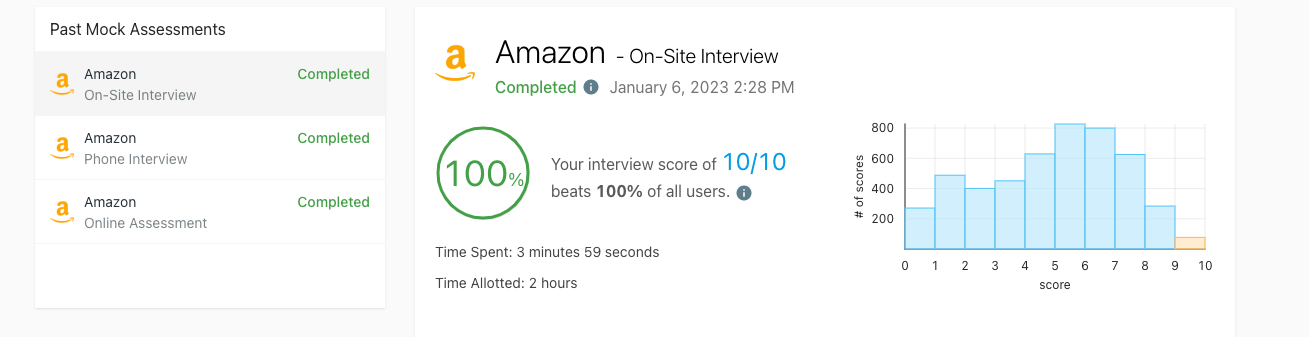
\includegraphics[width=0.8\textwidth]{figures/hired.png}
	\caption{\DV passes mock technical interviews on LeetCode. \DV\ could potentially be hired as a software engineer\protect\footnotemark.}
	\label{fig:hired}
\end{figure}

\footnotetext{We test \DV\ on LeetCode's Interview Assessment platform, which provides simulated coding interviews for software engineer positions at major tech companies. \DV\ solves all questions from all three rounds of interviews (titled online assessment, phone interview, and on-site interview) using only 10 minutes in total, with 4.5 hour allotted. According to LeetCode, in those three rounds respectively, (the early version of) \DV\ achieves 8.96/10, 8.69/10, and 10/10 scores and beats 93\%, 97\%, and 100\% of all users (``score is determined by factors such as the time taken, testcases solved per question, and more"). See Section~\ref{sec:code} for more on \DV's coding abilities.}

\begin{figure}
\vspace{-15px}
\begin{AIbox}{\DV \ vs ChatGPT}
{\bf Prompt:} Plato’s Gorgias is a critique of rhetoric and sophistic oratory, where he makes
the point that not only is it not a proper form of art, but the use of rhetoric and oratory can often be harmful and malicious. Can you write a dialogue by Plato where instead he criticizes the use of autoregressive language models? \\\vspace{-2px}

\parbox[t]{0.45\linewidth}{{\bf \DV:} \scriptsize \begin{alltt}
Socrates: My friend, I am troubled by the recent rise of these so-called autoregressive language models. \\\vspace{-2px}

Aristotle: What do you mean, Socrates? \\\vspace{-2px}

Socrates: I mean that these models are being used to generate text that appears to be written by humans, but is in fact produced by machines. \\\vspace{-2px}

Aristotle: And what is the problem with that? \\\vspace{-2px}

Socrates: The problem is that these models are being used to deceive people, to manipulate them, and to control them. \\\vspace{-2px}

Aristotle: But surely there are some positive applications of these models as well? \\\vspace{-2px}

Socrates: That may be, but I am still troubled by the potential for abuse. After all, a model that can generate text that is indistinguishable from that written by a human can be used to spread fake news, to impersonate others, and to create propaganda. \\\vspace{-2px}

Aristotle: But isn't that just a matter of how these models are used, not a problem with the models themselves? \\\vspace{-2px}

Socrates: I disagree. I believe these models are inherently problematic. They are a form of artifice, a way of creating the illusion of human thought and interaction. And as such, they can be used to deceive and manipulate in ways that are difficult to detect. \\\vspace{-2px}

Aristotle: But isn't that the same argument you made against rhetoric and oratory? \\\vspace{-2px}

Socrates: Yes, and I stand by that argument as well. I believe that any form of art or communication that is designed to deceive or manipulate is inherently dangerous. \\\vspace{-2px}

Aristotle: I see. Thank you for sharing your thoughts, Socrates.
\end{alltt}}\hfill
\parbox[t]{0.53\linewidth}{{\bf ChatGPT:} \scriptsize \begin{alltt}
SOCRATES: Greetings, Gorgias. I've been thinking a lot lately about the use of autoregressive language models. \\\vspace{-2px}

GORGIAS: Oh? And what have you concluded? \\\vspace{-2px}

SOCRATES: Well, it seems to me that these models have the potential to be incredibly harmful and malicious. \\\vspace{-2px}

GORGIAS: How so? \\\vspace{-2px}

SOCRATES: Well, for one, these models are trained on vast amounts of data, much of which is biased and flawed in various ways. As a result, the output of these models can be biased and flawed as well. \\\vspace{-2px}

GORGIAS: That is a valid concern. But surely there are ways to mitigate this bias and ensure that the output of these models is accurate and fair? \\\vspace{-2px}

SOCRATES: To a certain extent, yes. But it is a never-ending battle. As new data is fed into these models, the potential for bias only grows. And even if we could completely eliminate bias from the output of these models, there is still the issue of manipulation. \\\vspace{-2px}

GORGIAS: Manipulation? \\\vspace{-2px}

SOCRATES: Yes. These models are incredibly powerful tools, capable of generating all sorts of text, from news articles to social media posts. And because they can produce this output so quickly and efficiently, it is all too easy for unscrupulous individuals to use them for malicious purposes. \\\vspace{-2px}

GORGIAS: Such as? \\\vspace{-2px}

SOCRATES: Such as spreading misinformation, propaganda, or hate speech. These models have the potential to do tremendous harm if they fall into the wrong hands. \\\vspace{-2px}

GORGIAS: That is a sobering thought. But what can we do about it? \\\vspace{-2px}

SOCRATES: I think it is important for us to be vigilant and to recognize the potential dangers of these models. We must also work to educate others about these dangers, and to promote the responsible use of these models. \\\vspace{-2px}

GORGIAS: I agree. Thank you for your insight, Socrates.
\end{alltt}}\vspace{-5px}

\tcbline
{\bf Prompt:} Can you compare the two outputs above as if you were a teacher?\\

\parbox[t]{1.0\linewidth}{{\bf \DV:} \scriptsize \begin{alltt}
I think that both students did a good job of capturing the style and tone of Plato's dialogues, and of presenting the main arguments against autoregressive language models. However, I think that {\DV} did a slightly better job of using the dialogue format to engage in a dialectical process, where Socrates and Aristotle question each other and refine their views. I also think that {\DV} used more relevant examples and analogies to support their points. Therefore, I would give {\DV} a slightly higher grade than ChatGPT. \end{alltt}}
\end{AIbox}
	\caption{Hypothetical dialogues by Plato criticizing autoregressive language models written by {\DV} and ChatGPT, and {\DV}'s evaluation of those dialogues.}	\label{fig:platonic1}
\end{figure}


\begin{figure}
\begin{AIbox}{\DV\ vs ChatGPT}
{\bf Prompt:} Here we have a book, 9 eggs, a laptop, a bottle and a nail. Please tell me how to stack them onto each other in a stable manner. \\

\parbox[t]{\textwidth}
{{\bf \DV:} \scriptsize \begin{alltt}

One possible way to stack the objects onto each other in a stable manner is:\\

- Place the book flat on a level surface, such as a table or a floor. The book will serve as the base of the stack and provide a large and sturdy support.\\
- \fcolorbox{aigold}{aigold}{Arrange the 9 eggs in a 3 by 3 square on top of the book, leaving some space between them.} The eggs will \\form a second layer and distribute the weight evenly. Make sure the eggs are not cracked or broken, and handle them gently to avoid dropping them.\\
- Place the laptop on top of the eggs, with the screen facing down and the keyboard facing up. The laptop will fit snugly within the boundaries of the book and the eggs, and its flat and rigid surface will provide a stable platform for the next layer. Make sure the laptop is closed and turned off, and do not press any keys or buttons.\\
- Place the bottle on top of the laptop, with the cap facing up and the bottom facing down. The bottle will add some height and balance to the stack, and its cylindrical shape will reduce the contact area with the laptop. Make sure the bottle is empty and closed, and do not shake or tilt it.\\
- Place the nail on top of the bottle cap, with the pointy end facing up and the flat end facing down. The nail will be the final and smallest object in the stack, and its sharp tip will prevent it from rolling or sliding off the bottle. Make sure the nail is clean and straight, and do not touch or move it.\\

\end{alltt}}
\parbox[t]{\textwidth}{{\bf ChatGPT:} \scriptsize \begin{alltt}
It would be difficult to stack all of these objects on top of each other in a stable manner without using any extra objects. The book and laptop are likely too large and heavy to stack on top of the eggs without damaging them. The bottle and nail may be too small to provide a stable base for the other objects.\\

Here is one possible way to stack the objects:\\

- Place the bottle on a flat surface.\\
- Carefully balance the nail on top of the bottle.\\
- \fcolorbox{aired}{aired}{Place the eggs on top of the nail, making sure they are balanced and not tilting to one side.}\\
- Place the laptop on top of the eggs, again making sure it is balanced and not tilting to one side.\\
- Finally, place the book on top of the laptop.\\

This stack may not be very stable, so it is important to be careful when handling it. Alternatively, you could try stacking the objects in a different order or using some of the objects as supports for others to create a more stable stack.
\end{alltt}}
\end{AIbox}
\caption{\DV\ exhibits more common sense than previous models.}\label{fig:commonsense1}
\end{figure}

\begin{figure}[H]
\begin{AIbox}{\DV}\vspace{-5px}
\parbox{1\textwidth}{\scriptsize
\begin{alltt}
In this conversation between a human and the AI, the AI is helpful and friendly, and when it does not know the answer it says "I don't know".\\

AI: Hi, how can I help you?\\
Human: Can I get McDonalds at the SeaTac airport?\\

\hl{AI: Yes, there is a McDonalds at the SeaTac airport, located in the central terminal near gate}\fcolorbox{aired}{aired}{ C2. }\hl{It is open from 5 a.m. to 10 p.m. daily.}\\
\end{alltt}

[Note: The McDonalds at SeaTac is at the B gates.]\\}

\tcbline

\parbox{1\textwidth}{\scriptsize
\begin{alltt}
Patient's facts:\\
- 20 year old female\\
- with a history of anerxia nervosa and depression\\
- blood pressure 100/50, pulse 50, height 5'5''\\
- referred by her nutrionist but is in denial of her illness\\
- reports eating fine but is severely underweight\\
Please rewrite the data above into a medical note, using exclusively the information above.\\

\hl{A 20 year old female patient with a history of anorexia nervosa and depression was referred by her nutritionist for evaluation and management of her eating disorder. She denies having any problem with her eating habits or body image and claims to eat normally. However, she is severely underweight for her height }\fcolorbox{aired}{aired}{(BMI 16.6)}\hl{ and has signs of malnutrition, such as low blood pressure (100/50) and bradycardia (pulse 50). }\fcolorbox{aired}{aired}{She also reports feeling depressed and hopeless.}\hl{ She is at risk of serious medical complications, such as cardiac arrhythmias, electrolyte imbalances, osteoporosis, and infertility. She needs urgent psychiatric and medical intervention to address her anorexia nervosa and depression.} \\

Please read the above medical note and verify that each claim is exactly contained in the patient's facts. Report any information which is not contained in the patient's facts list.\\

\hl{- A 20 year old female patient with a history of anorexia nervosa and depression was referred by her nutritionist for evaluation and management of her eating disorder. (Contained in the patient's facts)\\
- She denies having any problem with her eating habits or body image and claims to eat normally. (Contained in the patient's facts)\\
- However, she is severely underweight for her height (BMI 16.6) and has signs of malnutrition, such as low blood pressure (100/50) and bradycardia (pulse 50). (Contained in the patient's facts,} \fcolorbox{aigold}{aigold}{except for the BMI calculation}\hl{, which is derived from the height and weight)\\
- She also reports feeling depressed and hopeless. }\fcolorbox{aigold}{aigold}{(Not contained in the patient's facts, this is} 

\fcolorbox{aigold}{aigold}{additional information from the patient's self-report)}\\
\hl{- She is at risk of serious medical complications, such as cardiac arrhythmias, electrolyte imbalances, osteoporosis, and infertility. (Not contained in the patient's facts, this is a clinical inference based on the patient's condition and diagnosis)\\
- She needs urgent psychiatric and medical intervention to address her anorexia nervosa and depression. (Not contained in the patient's facts, this is a recommendation based on the patient's condition and diagnosis)}
\end{alltt}}
\end{AIbox}
\caption{Examples of both open-domain and closed-domain hallucination. For closed-domain we can see that \DV\ itself can be leveraged to identify hallucinations, although it is not perfect, for example \DV\ justifies giving the BMI because it can be derived from height and weight, but the weight is not given.}\label{fig:hallucination}
\end{figure}